% SIAM Article Template
\documentclass[review,onefignum,onetabnum]{siamonline190516}

% Information that is shared between the article and the supplement
% (title and author information, macros, packages, etc.) goes into
% ex_shared.tex. If there is no supplement, this file can be included
% directly.

% Packages and macros go here
\usepackage{lipsum}
\usepackage{amsfonts}
\usepackage{graphicx}
\usepackage{epstopdf}
\usepackage{algorithmic}
\usepackage{tikz}
\usepackage{cite}
\usepackage[latin1]{inputenc}
\usetikzlibrary{trees}
\usetikzlibrary{matrix,positioning,quotes}
\ifpdf
  \DeclareGraphicsExtensions{.eps,.pdf,.png,.jpg}
\else
  \DeclareGraphicsExtensions{.eps}
\fi

% Prevent itemized lists from running into the left margin inside theorems and proofs
\usepackage{enumitem}
\setlist[enumerate]{leftmargin=.5in}
\setlist[itemize]{leftmargin=.5in}

% Add a serial/Oxford comma by default.
\newcommand{\creflastconjunction}{, and~}

% Used for creating new theorem and remark environments
\newsiamremark{remark}{Remark}
\newsiamremark{hypothesis}{Hypothesis}
\crefname{hypothesis}{Hypothesis}{Hypotheses}
\newsiamthm{claim}{Claim}

% Sets running headers as well as PDF title and authors
\headers{Faster network motif discovery by counting isomorphic subtrees}{J. Grochow, T. Tohme}

% Title. If the supplement option is on, then "Supplementary Material"
% is automatically inserted before the title.
\title{Faster network motif discovery by counting isomorphic subtrees\thanks{Submitted to the editors on DATE
\funding{During this work, JAG was partially funded by NSF grant DMS-1622390, and TT was funded by J. A. Grochow startup funds.}}}

% Authors: full names plus addresses.
\author{Joshua A. Grochow\thanks{Departments of Computer Science and Mathematics, University of Colorado, Boulder
  (\email{jgrochow@colorado.edu}).}
\and Tarek Tohme\thanks{Department of Computer Science, University of Colorado, Boulder
  (\email{tpt00@mail.aub.edu}).}
}

\usepackage{amsopn}
\DeclareMathOperator{\diag}{diag}

% Optional PDF information
\ifpdf
\hypersetup{
  pdftitle={Faster network motif discovery by counting isomorphic subtrees},
  pdfauthor={J. Grochow, T. Tohme}
}
\fi

% The next statement enables references to information in the
% supplement. See the xr-hyperref package for details.

%\externaldocument{ex_supplement}

% FundRef data to be entered by SIAM
%<funding-group specific-use="FundRef">
%<award-group>
%<funding-source>
%<named-content content-type="funder-name"> 
%</named-content> 
%<named-content content-type="funder-identifier"> 
%</named-content>
%</funding-source>
%<award-id> </award-id>
%</award-group>
%</funding-group>

\begin{document}

\maketitle

% REQUIRED
\begin{abstract}
  We develop a new algorithm for counting the number of subgraphs of a network isomorphic to a given query graph (\#\textsc{SubgraphIsomorphism}), motivated by network motif search. High-degree vertices (hubs), common in real-world networks, contribute to a combinatorial explosion in the number of subgraphs, making existing motif search algorithms intractable for motif sizes greater than 7 on a wide variety of networks of interest. Our procedure leverages the $k$-core decomposition and a novel subtree-counting technique to quickly scan the periphery of a network. These two innovations make our algorithm significantly faster than its predecessors in practice, especially as most real-world networks have a relatively large periphery. We prove that \#\textsc{RootedSubtreeIsomorphism} is \textbf{\#P}-complete via a reduction from counting bipartite matchings. We provide analytic upper bounds on our algorithm's execution time, and evaluate its performance on 11 real-world networks of varying topologies.
\end{abstract}

% REQUIRED
\begin{keywords}
  network motifs, subgraph isomorphism, $k$-core decomposition
\end{keywords}

% REQUIRED
\begin{AMS}
  05C85, 05C30, 05C60
\end{AMS}

\section{Introduction}

Networks are useful abstractions for studying structural patterns and properties in many types of systems
\cite{strogatz2001exploring, newman2018networks}. One way to study such patterns is by identifying repetitions of certain subnetworks, following the reasoning that in many systems, the frequent occurrence of a ``module" is an indicator of its importance in the function of the system. Patterns in a network that appear with statistically significant frequency with respect to a null model (an appropriately defined random network) are called \emph{network motifs} \cite{milo2002network}. Examples of networks where motifs have been studied include class diagrams in software architecture \cite{valverde2005network}, brain networks \cite{sporns2004motifs}, transcriptional regulation networks \cite{shen2002network} and many more \cite{ohnishi2010network, albert2004conserved, paulau2015motif, itzkovitz2005coarse}.

Since their introduction \cite{milo2002network}, an active line of research has been dedicated to the design of algorithms that search for such motifs ever more efficiently. Most of these algorithms fall under one of two categories: network-centric algorithms, in which all \cite{milo2002network, kashani2009kavosh, li2018mtmo} or a sample \cite{kashtan2004efficient, wernicke2006fanmod} of size-k subgraphs of a given network are enumerated, and motif-centric algorithms \cite{omidi2009moda, grochow2007network} in which size-k graphs are enumerated \emph{a priori} and mapped onto a network one by one. Typically in the former category, after enumeration, subgraphs are grouped into isomorphic equivalence classes and their frequencies are then calculated or estimated. Two of the advantages of motif-centric approaches are the possibility of searching for the instances of a single subgraph in a network, and the reduced cost of computing isomorphisms for each subgraph incurred in the classification task of network-centric algorithms. Additional ideas such as symmetry-breaking \cite{grochow2007network} and expansion trees \cite{omidi2009moda} have enabled further speedups, making it possible to search for all subgraphs up to size 8, and individual subgraphs up to size 30 \cite{grochow2007network}. The g-trie, introduced in \cite{ribeiro2010g}, is an efficient data structure that enables the search for any set of subgraphs, taking advantage of the similarity between subgraphs in that set. This minimizes the cost of redundant searches incurred by motif-centric approaches, which execute as many queries as there are subgraphs, disregarding their potential similarity, while eliminating the unnecessary isomorphism checks of network-centric subgraph enumeration. This method used in combination with symmetry-breaking produces a vast improvement compared with pre-existing approaches \cite{ribeiro2014g}. Additional techniques have included focusing only on tree motifs \cite{li2018mtmo}, parallelizing subgraph enumeration \cite{shao2014parallel} or subgraph mapping \cite{lin2016network}.

A few remarks serve to lay out our strategy for an improved motif search algorithm. First, we note that existing approaches to motif search all operate by either enumerating or mapping \emph{instances} of subgraphs inside a network. In principle, to discover motifs it would suffice to count all subgraphs of a network, rather than list them. The counting version of the subgraph isomorphism problem, \#\textsc{SubgraphIsomorphism}, asks how many subgraphs of a graph $G$ are isomorphic to another graph $H$. Algorithms for \#\textsc{SubgraphIsomorphism} include \cite{fomin2012faster} and \cite{alon2008biomolecular}. The latter color-coding technique achieves polynomial time when counting non-induced subgraphs of bounded treewidth, provided $|H| = O(log(|G|)$. However it was recently proved \cite{curticapean2014complexity} that boundedness of the vertex cover number of $H$ is the only condition that guarantees tractability for \#\textsc{SubgraphIsomorphism}. Regardless of asymptotic behavior, counting subgraphs has the potential to be faster than listing them, owing to the use of clever counting techniques and to the memory access and storage overhead when large numbers of instances are involved. The ESCAPE algorithm \cite{pinar2017escape}, which manages to count all size-5 subgraphs orders of magnitude more efficiently than predecessors, is a testimony to this.

Another issue with existing algorithms is that none of them account for the difference in runtime incurred by different subgraph topologies. Early on in the investigation of network motifs, it was suggested \cite{itzkovitz2003subgraphs} that certain subgraphs could contribute disproportionately more to the runtime of motif search because of combinatorial explosions in the number of times they appear in a network. A good example is the star graph of size $k$, of which there are $\binom{n-1}{k-1}$ instances in a star graph of size $n \geq k$.

Lastly, scale-free networks are known to possess large hierarchically structured hubs \cite{barabasi2001deterministic} which can quickly make the motif search problem intractable in the contexts where such networks show up. Putting aside the discussion of how ubiquitous scale-free networks really are \cite{broido2019scale}, biological networks, where investigations of network motifs originated, often also contain prohibitively large hubs \cite{prvzulj2004modeling} whether their degree distributions are scale-free, geometric, or log-normal. As we will check experimentally, the runtime of motif search can even be dominated by a single star motif while searching among hundreds or thousands of motifs, especially when the target network contains large hubs.

Taking into account the above remarks, we make \#\textsc{SubgraphIsomorphism} our focus in the present paper, and take advantage of both motif and network topology to accelerate subgraph counting. We build on Grochow-Kellis \cite{grochow2007network} to design a subgraph-counting algorithm that leverages tree and hub structure in a network. Our main contribution consists in separating each of the network and the query into two subsets using the $k$-core decomposition: the ``periphery", which contains all the low-connectedness nodes, and the more interconnected nodes, which can be viewed as ``the core". A key feature of this decomposition is that it guarantees that the periphery consists entirely of trees. This enables us to run the peripheries of both network and query through a fast subtree-counting algorithm, saving considerable time compared with standard motif search procedures. In addition, the $k$-core decomposition offers a powerful early abort for motif search; the \emph{coreness} of a vertex imposes a strong constraint on the possible isomorphisms that can map a query graph to a target network, allowing our algorithm to waste less time trying out mappings that do not yield valid instances. Complementing this result, we show that \#\textsc{RootedSubtreeIsomorphism}, where the network $G$ and query $H$ are rooted unlabeled trees, is \textbf{\#P}-complete. This suggests that, although our speed-ups in subtree counting are only heuristic, that one should not expect significantly improved worst-case bounds for the subtree counting portion of our algorithm.

\paragraph{Organization} In \Cref{sec:subtrees} we make the notions of core and periphery rigorous, provide an algorithm for subtree-counting and analyze its time complexity. \Cref{sec:main} introduces our main algorithm and provides an analytic treatment of its performance. We then test the algorithm on a corpus of 8 real networks, and relate its empirical performance to several key network statistics in \Cref{sec:experiments}. In \Cref{sec:discussion} we discuss the impact of subtree-counting and queries of high coreness on the computational complexity of motif search. We conclude in \Cref{sec:conclusion}.


\section{Counting subtrees in the $1$-shell}
\label{sec:subtrees}
\subsection{Background on the k-core decomposition}
\label{subsec:kcore}
The $k$-core decomposition \cite{kong2019k} is a procedure that reveals the ``core-periphery" structure of a given network. The k-core of a graph $G$ is the (unique) maximal subgraph $K$ such that every vertex in $K$ has at least $k$ neighbors in $K$. The \emph{$k$-shell} is the set of vertices in the $k$-core that are not part of the $k+1$-core. A vertex inside the $k$-shell is said to be of \emph{coreness k.} The $k$-core decomposition can be carried out in linear time as follows: remove all vertices of degree $1$ until there are none left, including vertices whose degree becomes at most one during this removal process. Those vertices constitute the 1-shell. Make additional passes removing all vertices of degree at most $k$ at each pass, labeling each vertex with its coreness $k$.

For graphs that have a nonempty $2$-core, the 1-shell consists entirely of trees, each of whose root belongs to the 2-core.
%\textbf{(add sketch)}
To see why, notice that no tree can contain a nontrivial subgraph where every vertex is of degree 2 or more. Performing a $k$-core decomposition on $H$ and $G$ reveals these peripheral trees, if they exist. By selecting one root at a time from each of $H$ and $G$'s 1-shell trees, we can then run a subtree-counting algorithm as a subroutine to any standard motif-centric algorithm. We build on the Grochow-Kellis symmetry-breaking algorithm \cite{grochow2007network}, but in principle our subtree-counting technique can be used with any standard motif-centric algorithm. In practice, there are subtleties of implementation that have to do with with symmetry-breaking and the 1-shell/2-core boundary that need to be addressed, and will be discussed in \cref{sec:boundary}. In the following we discuss the computational complexity of subtree-counting and motivate its use in the context of motif search.

\subsection{Description of the subtree-counting algorithm}
The permanent of an $m \times n$ matrix $A = (a_{ij})$ is defined as
\begin{equation}\label{eq:permanent}
  per(A) = \sum_{\sigma \in \Sigma(m,n)} \prod_{i=1}^{n}a_{i,\sigma(i)}
\end{equation}
where $\Sigma(m,n)$ is the set of all $m$-permutations of the index set. In a weighed bipartite graph $B$ with weighed $m \times n$ adjacency matrix $W = (w_{ij})$, if we define the weight of a matching $s$ as the product of the weights of all its edges

\begin{equation}\label{eq:weighed_bipartite}
  w(s) = \prod_{i=1}w_{i,s(i)}
\end{equation}
then the permanent of $W$ is the sum of the weights of all matchings of $B$. If we assign the weight of an edge $(u,v)$ to be the number of matchings between $T_u$ and $S_v$, the permanent of $W$ becomes the total number of instances of $T$ in $S$.

If the roots of trees $\{T,S\}$ have $k$ and $l$ children respectively, we need to compute $\binom{l}{k}$ permanents of $(k \times k)$ matrices to count all instances of $T$ in $S$. Hubs that appear in trees can make $\binom{l}{k}$ a very large number, and permanents of $k \times k$ matrices can be expensive to calculate when $k$ is large. Note that these computations happen for every non-leaf vertex of $T$, as we elaborate below. The following lemma points to a simplification that solves this issue.

\begin{lemma}
\label{lem:simplified_per}
  Let $B = (L, R, W)$ be a directed bipartite graph with an $m \times n$ weighed adjacency matrix $W = (w_{ij})$, and edge direction $(l, r)$, $\forall (l, r) \in L \times R$. If there exists a set $P \subseteq L$ such that $\forall u \in P$, deg$(u) = |R|$ and $\forall (u, v) \in S\times R,$ $w_{uv} = 1$, then
  \begin{equation}
  	per(W) = per(W') \times \binom{|R| - |L \setminus P|}{|P|}
  \end{equation}
where $W' = (w'_{ij})$ is the submatrix of $W$ with entries of weight $w_{ij} > 1$. In other words, if $B$ is the bipartite graph representing the number of matchings between two rooted trees $T$ and $S$, $P$ corresponds to the depth-1 vertices of $T$, and their contribution to the total number of matchings is the binomial coefficient in the above expression. $per(W')$ counts the matchings of $T$'s rooted subtrees of depth greater than 1 in $S$.
\end{lemma}

\begin{proof}
$W$ has the form
\begin{equation}
W = 
\begin{pmatrix}
	1 & 1 \\
	0 & W'
\end{pmatrix}
\end{equation}
where $W'$ is of dimension $m' \times n'$, and $0$ and $1$ are respectively the all-zeros and all-ones matrices of appropriate dimension.

\begin{align*}
  per(W) & = \sum_{\sigma \in \Sigma(m, n)} \prod_{i=0}^{m-1} w_{i,\sigma(i)} \\
  		 & = \sum_{\sigma \in \Sigma(m, n)} \Bigg[ \prod_{i=m-m'}^{m-1} w'_{i,\sigma(i)} \Big(\sum_{\sigma \in \Sigma(m, n)} \prod_{j=0}^{m-m'-1} w_{j,\sigma(j)} \Big) \Bigg] \\
		 & = \binom{n-m'}{m-m'}\times per(W')
\end{align*}
Noticing that $|R| = n$, $|L| = m$, and $|L\setminus P| = m'$ leads to the result.
\end{proof}

We use the above to propose a subtree-counting algorithm that achieves drastic speedup when compared with regular motif search algorithms running on trees. We make use of Ryser's formula \cite{ryser1963combinatorial} as a black box to compute permanents, but more efficient formulas could easily be inserted in our algorithm when they become available.

\begin{algorithm}
\caption{\textsc{CountRootedSubtrees}$(T, S, t, s, D)$}
\label{alg:buildtree}
\begin{algorithmic}
\STATE{treeChildrenT := $\{i | deg(i) > 1 \enspace \forall i \in t$.children\}}
\STATE{treeChildrenS := $\{i | deg(i) > 1 \enspace \forall i \in s$.children\}}
\STATE{starChildrenT := $\{i | deg(i) = 1 \enspace \forall i \in t$.children\}}
\STATE{subtreesPreorderStrings := $\{D[i] \enspace \forall i \in $ treeChildrenT\}}
\STATE{equivalenceClassSizes := \{countStringsEqualTo[$k$] $\enspace \forall k \in$ subtreesPreorderStrings\}}
\STATE{multiplicity := 1}
\STATE{}

\FOR{$n$ in equivalenceClassSizes}
\STATE{multiplicity := multiplicity $\times \, n!$}
\ENDFOR
\STATE{}

\IF{$t$.children = $\emptyset$}
\RETURN 1
\ELSIF{treeChildrenT = $\emptyset$}
\STATE{$n := t$.children.size}
\STATE{$k := s$.children.size}
\RETURN $\binom{n}{k}$
\ENDIF
\STATE{}

\FOR{$u$ in treeChildrenT}
\FOR{$v$ in treeChildrenS}
\STATE{$T_u$ := detachTree($T, u, t)$} \quad //the ``downward-facing" subtree of $T$ rooted at $u$
\STATE{$S_v$ := detachTree($S, v, s)$}
\STATE{$k$ := \textsc{CountRootedSubtrees}($T_u, S_v, u, v, D$)}
\STATE{$W'[u][v]$ := $k$}
\ENDFOR
\ENDFOR
\STATE{}

\STATE{$n := s$.children.size $-$ treeChildrenT.size}
\STATE{$k := $starChildrenT.size}
\RETURN $(permanent(W') \div$ multiplicity $) \times \binom{n}{k}$
\end{algorithmic}
\end{algorithm}

\cref{alg:buildtree} counts all the rooted instances of an unlabeled rooted tree $T$ inside an unlabeled rooted tree $S$, where the roots of both trees are given by $t$ and $s$ respectively. $D$ is a dictionary that stores at key $u$ the preorder traversal string of the subtree of $T$ rooted at $u$ for all nodes $u \in T$ (here we abuse the term ``subtree" by having it refer to the subgraph of $T$ that contains $u$ and all its descendants relative to the root of $T$).

Among $T$'s and $S$'s depth-1 vertices, the subset of those that form a star graph along with the root (i.e. those of degree 1) are called starChildren. The remaining vertices are the treeChildren. By \cref{lem:simplified_per}, we can compute matchings among the treeChildren of $T$ and $S$ separately, and obtain the matchings between starChildrenT and the children of $s$ from the binomial factor.

We are interested in counting only one copy of $T$ inside $S$ for each one of $T$'s automorphism classes, since we are dealing with unlabeled trees where symmetries do not matter. To account for this, the algorithm starts by listing the preorder strings of the subtrees of $T$ rooted at $T$'s treeChildren, and grouping the identical strings among that list into equivalence classes (recall that a preorder traversal uniquely determines an unlabeled tree, up to symmetry). There are $n!$ possible permutations of the elements of an equivalence class of subtrees, whence the correction factor \emph{multiplicity}.

Next, the algorithm checks for the two base cases, where $T$ consists of only one node with no children, and where $T$ has no treeChildren. Otherwise, it loops through every pair of subtrees ($T_u$, $S_v$) of depth greater than 1 and recursively counts the instances of $T_u$ in $S_v$, storing the count in a matrix $W'$ at entry $[u][v]$. This is equivalent to constructing a directed bipartite graph and assigning a weight $k$ to edge $(u, v)$. \\
Finally, the permanent of $W'$ is computed using Ryser's formula:
\begin{equation}
	perm(W') = \sum_{k=0}^{n-1}(-1)^k\Sigma_k
\end{equation}
where $\Sigma_k$ is obtained by summing the products of the row-sums of $A_k$, the matrix obtained by deleting $k$ rows from $W'$, for all combinations of rows. The worst-case time complexity of using Ryser's formula for the permanent is $O(2^{n-1}n^2)$ \cite{ryser1963combinatorial}. However, to get an idea of how much faster \cref{alg:buildtree} is than regular motif search over trees in practice, see \cref{sec:experiments}.

\subsection{Complexity of counting subtrees}
% deterministic poly-time verifier of witnesses definition for counting TMs. \cite{valiant1979complexity}
We refer to standard textbooks such as Arora \& Barak \cite{arora2009computational} for background on \textbf{\#P} and \textbf{\#P}-completeness. Here we remark that \textbf{\#P}-complete problems are at least as hard, and though to be significantly harder, than NP-complete problems, so a \textbf{\#P}-completeness result for a counting problem indicates strongly that we should not expect a subexponential-time algorithm to exist. In this section, we prove such a result for the following problem. \\
\begin{quotation}
\noindent \#\textsc{RootedSubtreeIsomorphism} \\
Input: Two rooted trees $T$ and $S$ with their respective roots $t$ and $s$. \\
Output: The number of isomorphisms $\phi$ that map all of $T$ to a subset of $S$, up to the automorphisms of $T$, and verify $\phi(t) = s$. \\
\end{quotation}
We proceed via a reduction from the known \textbf{\#P}-complete problem of \#\textsc{PerfectMatchings}. We include the definition of membership in \textbf{\#P} \cite{arora2009computational} below for convenience. 
\begin{definition}
	A function $f : \{0,1\}^* \mapsto \mathbb{N}$ is in \textbf{\#P} if there exists a polynomial-time Turing Machine $M$ such that for any $x \in \{0,1\}^*$, $f(x)$ is the number of polynomial-size certificates $y$ satisfying $M(x, y) = 1$.
\end{definition}
That \#\textsc{RootedSubtreeIsomorphism} is in \textbf{\#P} is easy to verify: at each level of both $T$ and $S$, we sort the children of each vertex by degree and construct the unique map $\phi$ between $T$ and a subtree of $S$ which preserves that ordering, with $\phi(t) = s$. Namely,
\begin{equation}
\forall u_1,u_2 \in T,  deg(u_1) < deg(u_2) \iff deg(\phi(u_1)) < deg(\phi(u_2))
\end{equation}
We then loop through each $u_i \in T$, and add adjacent vertices $\{v_{ij}\}$ to $u_i$ until $deg(u_i) = deg(\phi(u_i))$. The index $j$ indicates the position of the adjacent vertex in the sorted list of $u_i$'s neighbors. This ensures that the resulting tree $T'$ is isomorphic to $S$. The sequence of $v_{ij}$'s is a polynomial-size certificate that uniquely determines the instance of $S$ that $T$ maps to, so there are as many such sequences as there are instances of $T$ in $S$.

We write $T \preceq S$ if there exists a root-preserving isomorphism between tree $T$ and a subtree of $S$, and $T \preceq ! \, S$ if such an isomorphism is unique up to the symmetries of $T$, i.e. there is a unique rooted subtree of S that is rooted-isomorphic to T (note that in a tree, all subgraphs are induced).

\begin{figure}[tphb]\label{fig:equiv_example}
	\centering
	\tikzstyle{level 1}=[level distance=2cm, sibling distance=3.2cm]
	\tikzstyle{level 2}=[level distance=2cm, sibling distance=1cm]
	\tikzstyle{level 3}=[level distance=2cm, sibling distance=0.4cm]
	
	\tikzstyle{end} = [circle, minimum width=3pt,fill, inner sep=0pt]
	\begin{center}
	\begin{tikzpicture}[grow=right, scale=0.5, baseline=-2.1cm]
    \node[end, label=left:{$T$}] {}
        child {
            node[end, label=below:{$T_{u_3}$}] {}        
            child {
                    node[end] {}
                    child {
                    	node[end, label=right:{}] {}
                    	edge from parent
                    	node[above] {}
                    	node[below] {}
                	}
                    edge from parent
                    node[above] {}
                    node[below] {}
                }
                child {
                    node[end, label=right:{}] {}
                    child {
                    	node[end, label=right:{}] {}
                    	edge from parent
                    	node[above] {}
                    	node[below] {}
                	}
                    edge from parent
                    node[above] {}
                    node[below] {}
                }
                child {
                    node[end] {}
                    child {
                    	node[end, label=right:{}] {}
                    	edge from parent
                    	node[above] {}
                    	node[below] {}
                	}
                    edge from parent
                    node[above] {}
                    node[below] {}
                }
            edge from parent         
                node[above] {}
                node[below] {}
        }
        child {
            node[end, label=above:{$T_{u_2}$}] {}        
            child {
                    node[end, label=below:{}] {}
                    child {
                    	node[end, label=right:{}] {}
                    	edge from parent
                    	node[above] {}
                    	node[below] {}
                	}
					child {
                    	node[end, label=right:{}] {}
                    	edge from parent
                    	node[above] {}
                    	node[below] {}
                	}
                    edge from parent
                    node[above] {}
                    node[below] {}
                }
                child {
                    node[end, label=above:{}] {}
                    child {
                    	node[end, label=right:{}] {}
                    	edge from parent
                    	node[above] {}
                    	node[below] {}
                	}
					child {
                    	node[end, label=right:{}] {}
                    	edge from parent
                    	node[above] {}
                    	node[below] {}
                	}
                    edge from parent
                    node[above] {}
                    node[below] {}
                }
            edge from parent         
                node[above] {}
                node[below] {}
        }
        child {
            node[end, label=above:{$T_{u_1}$}] {}        
            child {
                    node[end, label=right:{}] {}
                    child {
                    	node[end, label=right:{}] {}
                    	edge from parent
                    	node[above] {}
                    	node[below] {}
                	}
					child {
                    	node[end, label=right:{}] {}
                    	edge from parent
                    	node[above] {}
                    	node[below] {}
                	}
					child {
                    	node[end, label=right:{}] {}
                    	edge from parent
                    	node[above] {}
                    	node[below] {}
                	}
                    edge from parent
                    node[above] {}
                    node[below] {}
                }
            edge from parent         
                node[above] {}
                node[below] {}
        };
    \end{tikzpicture}
    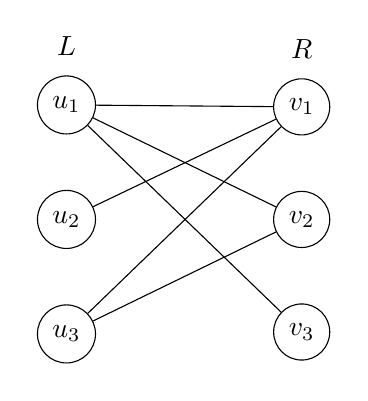
\begin{tikzpicture}[thin,amat/.style={matrix of nodes,nodes in empty cells,
      row sep=2em,
      nodes={draw,solid,circle,execute at begin node={$u_{\the\pgfmatrixcurrentrow}$}}},
      amat2/.style={matrix of nodes,nodes in empty cells,
      row sep=2em,
      nodes={draw,solid,circle,execute at begin node={$v_{\the\pgfmatrixcurrentrow}$}}},
      fsnode/.style={},
      ssnode/.style={}]
    
     \matrix[amat,nodes=fsnode,label=above:$L$] (mat1) {\\
     \\
     \\};
    
     \matrix[amat2,right=2cm of mat1,nodes=ssnode,label=above:$R$] (mat2) {\\
     \\ 
     \\};
    
     \draw  (mat1-1-1) edge (mat2-1-1)
     		(mat1-1-1) edge (mat2-2-1)
            (mat1-1-1) edge (mat2-3-1)
	        (mat1-2-1) edge (mat2-1-1)
	        (mat1-3-1) edge (mat2-1-1)
	        (mat1-3-1) edge (mat2-2-1);
	 
    \end{tikzpicture}
    \,\,
    \begin{tikzpicture}[grow=left, scale=0.5, baseline=-2.1cm]
    \node[end, label=right:{$S$}] {}
        child {
            node[end, label=above:{$S_{v_1}$}] {}        
            child {
                    node[end] {}
                    child {
                    	node[end, label=right:{}] {}
                    	edge from parent
                    	node[above] {}
                    	node[below] {}
                	}
					child {
                    	node[end, label=right:{}] {}
                    	edge from parent
                    	node[above] {}
                    	node[below] {}
                	}
					child {
                    	node[end, label=right:{}] {}
                    	edge from parent
                    	node[above] {}
                    	node[below] {}
                	}
                    edge from parent
                    node[above] {}
                    node[below] {}
                }
                child {
                    node[end, label=right:{}] {}
                    child {
                    	node[end, label=right:{}] {}
                    	edge from parent
                    	node[above] {}
                    	node[below] {}
                	}
					child {
                    	node[end, label=right:{}] {}
                    	edge from parent
                    	node[above] {}
                    	node[below] {}
                	}
                    edge from parent
                    node[above] {}
                    node[below] {}
                }
                child {
                    node[end] {}
                    child {
                    	node[end, label=right:{}] {}
                    	edge from parent
                    	node[above] {}
                    	node[below] {}
                	}
                    edge from parent
                    node[above] {}
                    node[below] {}
                }
            edge from parent         
                node[above] {}
                node[below] {}
        }
        child {
            node[end, label=above:{$S_{v_2}$}] {}        
            child {
                    node[end, label=right:{}] {}
                    child {
                    	node[end, label=right:{}] {}
                    	edge from parent
                    	node[above] {}
                    	node[below] {}
                	}
					child {
                    	node[end, label=right:{}] {}
                    	edge from parent
                    	node[above] {}
                    	node[below] {}
                	}
					child {
                    	node[end, label=right:{}] {}
                    	edge from parent
                    	node[above] {}
                    	node[below] {}
                	}
                    edge from parent
                    node[above] {}
                    node[below] {}
                }
                child {
                    node[end, label=right:{}] {}
                    child {
                    	node[end, label=right:{}] {}
                    	edge from parent
                    	node[above] {}
                    	node[below] {}
                	}
                    edge from parent
                    node[above] {}
                    node[below] {}
                }
                child {
                    node[end, label=right:{}] {}
                    child {
                    	node[end, label=right:{}] {}
                    	edge from parent
                    	node[above] {}
                    	node[below] {}
                	}
                    edge from parent
                    node[above] {}
                    node[below] {}
                }
            edge from parent         
                node[above] {}
                node[below] {}
        }
        child {
            node[end, label=below:{$S_{v_3}$}] {}        
            child {
                    node[end, label=right:{}] {}
                    child {
                    	node[end, label=right:{}] {}
                    	edge from parent
                    	node[above] {}
                    	node[below] {}
                	}
					child {
                    	node[end, label=right:{}] {}
                    	edge from parent
                    	node[above] {}
                    	node[below] {}
                	}
					child {
                    	node[end, label=right:{}] {}
                    	edge from parent
                    	node[above] {}
                    	node[below] {}
                	}
                    edge from parent
                    node[above] {}
                    node[below] {}
                }
            child {
                    node[end, label=right:{}] {}
                    edge from parent
                    node[above] {}
                    node[below] {}
                }
            child {
                    node[end, label=right:{}] {}
                    edge from parent
                    node[above] {}
                    node[below] {}
                }
            edge from parent         
                node[above] {}
                node[below] {}
        };
    \end{tikzpicture}
    \end{center}
  \caption{Graphical example of equivalence \cref{eq:bipartite_equiv}.}
\end{figure}

\begin{theorem}\label{thm:subtree_count}
  \#\textsc{PerfectMatchings} $\leq_T$ \#\textsc{RootedSubtreeIsomorphism}
\end{theorem}

\begin{proof}
Let $B = (L, R, E)$ be a bipartite graph where $L$ and $R$ are respectively the sets of left and right vertices, and $E \subseteq L \times R$ is the set of edges. We construct a tree $T_u$ for each vertex $u \in L$, and a tree $S_v$ for each $v \in R$ (see \cref{fig:equiv_example}), such that
\begin{equation}\label{eq:bipartite_equiv}
  (u,v) \in E \iff T_u \preceq! \, S_v
\end{equation}
We construct the $\{T_u\}_{u \in L}$ trees as follows: $\forall i \in \{1, \dots, |L|\}$, $T_{u_i}$ has $i$ depth-1 vertices, and each of those has $|L| - i + 1$ children. For the $\{S_v\}$ trees, $\forall j \in \{1, \dots, |R|\}$, $S_{v_j}$ has exactly $|L|$ depth-1 vertices. We then populate the children of those vertices by ``inserting" one copy of $T_{u_i}$ into $S_{v_j}$ if and only if $(u_i, v_j) \in E$; in other words, $i$ among $S_{v_j}$'s depth-1 vertices has at least $|L| - i + 1$ children, and the remaining $|L| - i$ depth-1 vertices have no children. This construction guarantees that at least one instance of $T_{v_i}$ appears in $S_{v_j}$ whenever $(u_i, v_j) \in E$.

To ensure that at most one instance of $T_{v_i}$ can appear in $S_{v_j}$ for any $i$ and $j$, we add a labeling for every depth-1 and depth-2 vertex (all leaf vertices and their parents) of both trees in the spirit of Grochow and Kellis' symmetry-breaking technique \cite{grochow2007network}. Namely, for all $j$, we add a unique label to each of the depth-1 and depth-2 vertices of $S_{v_j}$. Then, for all $i$, and for each of levels 1 and 2 in $T_{v_i}$, we find symmetry-breaking conditions by picking a vertex $n_0$ at random from that level (which by construction consists of an equivalence class of vertices all isomorphic to each other) and assigning to it the condition $L(n_0) < min(L(n_1), \dots, L(n_k))$. We do the same for all remaining vertices in that level. Any map from $T_{v_i}$ to $S_{v_j}$ induces a labeling on $T_{v_i}$, and there is a unique map that satisfies the conditions imposed on these labelings.

To complete the construction, on the left side of the bipartite graph we create a tree by adding an edge between a new root vertex $t$ and the root of $T_u$, for each $u \in L$. Every $T_u$ is now a subtree of the new tree $T$, rooted at a child vertex of $t$. Similarly, we create tree $S$ on the right side. This establishes a bijection between a matching of $B$ and a rooted subtree of $S$ isomorphic to $T$. The bijection is given as follows:
\begin{enumerate}
\item{Given a matching $\psi \in (L \times R)^{|L|}$ of $B$, for each $u \in L$, $T_{u}$ is isomorphic to exactly one subtree of $S_{\psi(u)}$, and the union of each of these subtrees along with the root $s$ constitutes the unique instance of $T$ that appears within $S$.}
\item{Given a rooted subtree $S' \subseteq S$ isomorphic to $T$, the matching consists of edges $(u_i,v_i) \in L \times R, i \in \{1,\dots,|L|\}$, each corresponding to a map between the subtree $S'_{v_i} \subseteq S'$ and $T_{u_i}$, the existence of which is guaranteed by the construction.}
\end{enumerate}
  
  Valiant has shown that counting the number of perfect matchings is \textbf{\#P}-complete \cite{valiant1979permanent}. Now if a Turing machine can query an oracle for \#\textsc{RootedSubtreeIsomorphism} on instance $(T, S)$, the answer is equal to the number of bipartite matchings in graph $B$, thus establishing the result.
\end{proof}

Like bipartite matching, this result is surprising considering that its corresponding decision problem, \textsc{RootedSubtreeIsomorphism}, is in \textbf{P}. We note that this result is different from the one proved by Goldberg and Jerrum in 2000 \cite{goldberg2000counting}, in which counting all rooted subtrees which are \emph{distinct} up to isomorphism within a given tree is proved \textbf{\#P}-complete, whereas our result concerns counting all rooted subtrees of a tree \emph{equivalent} up to isomorphism to a given tree (disregarding the symmetries of that tree).



\section{The subgraph-counting algorithm}
\label{sec:main}

\subsection{Boundary conditions}
\label{sec:boundary}
Recall from the introduction that our method consists in separating the 1-shell from the 2-core and performing subtree-counting on the former, then running a regular motif search algorithm on the latter. In doing so we must take care of a few boundary cases that arise at the interface between the 1-shell and the 2-core \textbf{(add figure to visualize 1-shell and 2-core)}. To see why, let $H = (C_H, P_H)$ be a query graph and $G = (C_G, P_G)$ be a network, where $C$ and $P$ refer respectively to the 2-core and the 1-shell. An instance of $H$ could appear ``halfway" between the 1-shell and the 2-core of $G$ such that only part of $P_H$ extends into $P_G$.  Because of this, to properly count every instance of $H$ in $G$, we must run each tree $T_H \in P_H$ as well as all of its subtrees through \cref{alg:buildtree}. By using the symmetry-breaking technique introduced in \cite{grochow2007network} on $T_H$, we can cut down the cost incurred by enumerating all possible subtrees by an amount proportional to the product of the number of symmetries at each level of trees of $P_H$.

On the flip side, another boundary condition provides us with a powerful early abort when searching for instances of $H$ inside $G$: suppose that $H$ appears halfway between $C_G$ and $P_G$, only this time $C_H$ extends partially into $P_G$. As we prove below, this cannot happen. In fact, it cannot happen between a $k$-core in $H$ and an $h$-shell in $G$ for any integers $h < k$ without violating induced isomorphism, which we require in the formal definition of ``an instance of $H$ inside $G$".

\begin{definition} \label{def:induced_iso}We say that an instance of $H = (V_H, E_H)$ appears in $G=(V_G, E_G)$ when there exists an induced isomorphism $\phi:V_H \mapsto V_G$ between the nodes of $H$ and those of $G$: 
\begin{equation}
\forall u,v \in V_H, \enspace (u,v) \in E_H \iff (\phi(u), \phi(v)) \in E_G
\end{equation}
\end{definition}

\begin{theorem}\label{thm:early_abort}
   For any $k$, a mapping between a vertex $v \in H$ of coreness $k$ onto a vertex $u \in G$ of coreness $h < k$ violates induced isomorphism between $H$ and $G$.
\end{theorem}

\begin{proof}
  First notice that a vertex $v$ in a graph's $k$-shell can have at most $k$ neighbors in the $k+1$-core. Otherwise, it wouldn't be removed when the $k$-core decomposition is making passes to remove vertices of degree at most $k$, and hence would not be part of the $k$-shell by definition. By the same reasoning, a vertex $u$ in the $k+1$-core must have at least $k+1$ neighbors inside the $k+1$-core. The above definition implies that an isomorphism that maps $u$ to $v$ should also map at least one of $u$'s $k+1$-core neighbors to a neighbor of $v$ in the $k$-shell. Proceeding by induction, we see that $v$ has at least $k+1$ neighbors, each of which has at least $k+1$ neighbors, and so on. Therefore $v$ must be in the $k+1$-core, a contradiction.
\end{proof}

We can use this fact to create an early abort by coreness: our algorithm should never bother to try to map a vertex in $H$ to another in $G$ with lesser coreness.

% why onion spectrum doesn't work as early abort by coreness

\subsection{Main result}
We build on the Grochow-Kellis symmetry-breaking algorithm, and refer to the function from their paper by the same name. \cref{alg:countsubgraphs} takes in two graphs $H$ and $G$, and returns the number of images of $H$ that appear in $G$. It starts by running a $k$-core decomposition on both graphs. Then, as in the Grochow-Kellis algorithm, it finds all automorphisms from $H$ onto itself by calling \textsc{FindSubgraphInstances($H, H$)} \cite{grochow2007network}, groups the nodes that map to each other in the same equivalence class and returns a representative node from each class. We abbreviate this behavior in the function \emph{findEquivalenceClassRepresentatives}. The symmetry-breaking conditions are also computed similarly as in \cite{grochow2007network}.


The next part of the algorithm consists in listing all the subtrees of the 1-shell of $H$, up to symmetry. This is done by the function \emph{enumerateSubtrees}, which stores them in the dictionary \emph{subtrees}, keyed by the nodes in $H$ at which they are rooted. It does this by again making use of symmetry-breaking, and listing only one tree from each equivalence class of symmetries.

\begin{algorithm}
\caption{\textsc{CountSubgraphs}$(H, G)$}
\label{alg:countsubgraphs}
\begin{algorithmic}
\STATE{//Initialization}
\STATE{kCoreDecompose(H)}
\STATE{kCoreDecompose(G)}
\STATE{$ECR_H$ := findEquivalenceClassesRepresentatives($H$)}
\STATE{$SBC_H$ := findSymmetryBreakingConditions($H$)}
\STATE{$f$ := initializeParitalMap}
\STATE{}
\STATE{//enumerating all subtrees in $H$'s 1-shell}
\FOR{$h$ in $ECR_H$}
	\IF{$h \in P_H$ OR $h$ is a root} %\quad //$P_H$ is the 1-shell of $H$
		\STATE{$T$ := detachTree($H, h$[, parent($h$)])}
		\STATE{subtrees[$h$] := enumerateSubtrees($T$, $h$)}
	\ENDIF
\ENDFOR
\STATE{}
\STATE{//counting subtrees in $G$'s 1-shell and boundary}
\FOR{$g$ in kCoreTraversalOrder($G$)}
	\IF{$g \in P_G$ AND $H$ is a tree}
		\STATE{$S$ := detachTree($G$, $g$, parent($g$))}
		\FOR{$h$ in $ECR_H$}
			\STATE{1ShellCount := \textsc{CountRootedSubtrees}($H, h, S, g$)}
		\ENDFOR
	\STATE{}
	\ELSIF{$g$ is a root}
		\STATE{$S$ := detachTree($G, g$)}
		\FOR{$h$ in $ECR_H$}
			\FOR{$T_h$ in subtrees[$h$]}
				\STATE{boundaryMultiplier := \textsc{CountRootedSubtrees}($T_h, h, S, g$)}
				\STATE{$f$.setMultiplier(boundaryMultiplier)}
				\STATE{$G$.markNodes($S$)}
				\STATE{\textsc{IsomorphicExtensions($f, H \backslash T_h, G, SBC_H$)}}
			\ENDFOR
		\ENDFOR
		\STATE{$G$.removeNodes($S$)}
	\ENDIF
\ENDFOR
\STATE{}
\STATE{//counting subgraphs in the 2-core}
\STATE{2CoreCount := count(\textsc{FindSubgraphInstances($H, G$)})}
\STATE{boundaryCount := $\prod_{f \in boundary} f$.getMultiplier}
\STATE{}
\RETURN 1ShellCount + boundaryCount + 2CoreCount

\end{algorithmic}
\end{algorithm}
The algorithm proceeds to count the subtrees of $H$ that appear in $G$'s 1-shell and at the boundary with its 2-core. It loops through all of $G$'s nodes in the same order as the $k$-core decomposition to quickly scan the 1-shell nodes and then remove them, making the subsequent 2-core search more tractable. We make use of the function $f$, which represents the partial isomorphism between a subset of $H$ and $G$ as the algorithm progresses in its search. For the boundary case, we associate each $f$ with a multiplier, which simply consists of a count of the number of subtrees that ``extend" from $f$ into the 1-shell of $G$. \textsc{IsomorphicExtensions} is a function introduced in \cite{grochow2007network} which incrementally extends $f$ one vertex at a time until it maps the entirety of $H$ onto a subset of $G$. By using the multiplier, we can initialize $f$ from a root of $G$ and let it expand inward into the 2-core, and use \textsc{CountRootedSubtrees} to count partial instances of $H$ in the 1-shell. At the end of the search, we multiply the number of instances found by \textsc{IsomorphicExtensions} by their individual multipliers to recover the total number of boundary instances. The vertices scanned by the subtree-counting routine are marked to prevent $f$ extending into the 1-shell. After all the 1-shell vertices are taken care of, they are removed and only the 2-core of $G$ remains.

Note that here we use a slightly modified version of \textsc{IsomorphicExtensions} that accounts for the early abort by coreness feature discussed above. Namely, when searching for an image vertex $g \in G$, \textsc{IsomorphicExtensions} first checks the coreness of $g$ to ensure that it is greater or equal than the coreness of its tentative preimage $h$.

\subsection{Upper bounds on runtime}
The subtree-counting algorithm works by recursively computing the number of matchings at each level of a query tree $T$ and a target tree $S$. To obtain an analytic upper bound on the number of steps in its execution, we count the total number of calls to \textsc{CountRootedSubtrees}, and multiply that by the worst-case runtime of computing the permanent of a weighed adjacency matrix. Note that in general such a matrix will not be square, which leads to an added binomial coefficient in the permanent's runtime contribution. This is because the permanent of a non-square matrix is the product of the permanents of each of its square submatrices.

The following is an approximate expression of the number of steps in \textsc{CountRootedSubtrees}' execution on trees $T$ and $S$ . $T'$ is the set of non-leaf vertices of $T$, $\phi$ is the root-preserving isomorphism mapping $T$ to a subtree of $S$, $m_u$ and $n_v$ are the number of children of vertices $u \in T$ and $v \in S$ respectively:

\begin{equation}
\label{eq:subtrees_upperbound}
f_{crs}(T, S) \approx \sum_{u \in T'} \binom{n_{\phi(u)}}{m_u} \times m_u^2 \times 2^{m_u - 1}
\end{equation}

By comparison, the Grochow-Kellis algorithm will test all $m$ vertices of $T$ with all $n$ vertices of $S$ up to symmetries of $T$.

\begin{equation}
\label{eq:gk_upperbound}
f_{gk}(T, S) \approx \frac{1}{|Aut(T)|}\binom{n}{m} = \frac{1}{|Aut(T)|}\binom{1+\sum_{u \in T'} n_{\phi(u)}}{1+\sum_{u \in T'} m_u}
\end{equation}

In the context of counting subgraphs, \textsc{CountRootedSubtrees} will be called once for each pair of non-leaf vertices in $H$ and roots in $G$. To factor in the speedup afforded by the coreness condition described in \cref{thm:early_abort}, let $m = |H|$ and $n = |G|$, let $m_K$, $n_K$ be the sizes of the $k$-cores of $H$ and $G$, and $R$ the number of roots in $G$. This gives an upper bound on the total runtime of the subgraph counting algorithm:

\begin{equation}
\label{eq:coreness_upperbound}
f_{cs}(H, G) \leq \frac{R}{|Aut(H)|} \times \sum_{T \subseteq P_H} f_{crs}(T, S) \times \binom{n_K}{m_K} \binom{n_{K-1} - m_K}{m_{K-1} - m_K} \dots \binom{n_2 - m_3}{m_2 - m_3}
\end{equation}

We compare this with an upper bound on the Grochow-Kellis algorithm's performance:

\begin{equation}
f_{gk}(H, G) \leq \frac{1}{|Aut(H)|}\binom{n}{m}
\end{equation}

\section{Real-data experiments}
\label{sec:experiments}

\subsection{Methods}
We implemented the Grochow-Kellis algorithm and \cref{alg:countsubgraphs} in Python 3.6 and ran them on a set of Intel Xeon E5-2680 v3 processors at 2.50GHz running Red Hat Enterprise Linux 7, from CU Boulder's RMACC supercomputer. Because each motif/network query is a computation that can be run on a separate processor, we made use of concurrency wherever possible. The runtimes we report in the following section are expressions of the total time taken for all concurrent processes summed together.

Using data from the communityFitNet corpus \cite{ghasemian2017evaluating} we tested a sample of 8 undirected networks of comparable sizes (around 150 vertices) spanning different topologies and categories of systems. We took care in our selection (by visual inspection) to make sure each network's topology was typical of the networks that represent the same type of system in the communityFitNet dataset. In each network we searched for all undirected graphs up to size 8 \textbf{see figure}. Informed by the upper bounds derived in the previous section, we then compared the speedup afforded by our algorithm to the following network statistics: size of the 1-shell, maximum degree and average non-leaf degree in the 1-shell, maximum and average coreness of 2-core, and maximum and average tree depth in 1-shell. We identified the first three statistics as being most predictive of a large performance improvement in our algorithm. We computed these statistcs for all 442 undirected networks from the communityFitNet corpus, highlighting those with large, dense 1-shells and peripheral hubs as potential applications for our algorithm. Finally, we tested three networks of around 1000 vertices, and demonstrate our algorithm's performance in querying all undirected graphs up to size 6.

\subsection{Results and discussion}
\label{sec:discussion}
%we show in (figure a) the distributions of maximum coreness and maximum peripheral hub degree for all size-6 undirected graphs. A side-by-side comparison of these distributions with their contributions to the runtime of GK on the Barrett & Helenurm network indicate that maximum peripheral hub degree is a much larger factor in the runtime.

\Cref{fig:runtime_comparison} shows our selection of 8 undirected networks along with network statistics we considered as potential indicators for our algorithm's improvement. \Cref{fig:lsample_comparison} shows runtimes on three larger networks for additional benchmarking. At first sight, the contribution of subtree-counting to our algorithm's speedup is more evident than that of early abort by coreness. We found that the speedup gained from queries of high maximal coreness is negligible compared with that of queries of high maximal hub degree (or star graphs). A hint to this lies in the fact that products of binomial coefficients of terms of a sum, such as in \cref{eq:coreness_upperbound}, are vastly larger than sums of binomial coefficients of terms of a sum, as in \cref{eq:subtrees_upperbound}, but both are much smaller than binomial coefficients involving the entire sum (\cref{eq:gk_upperbound}).

Our aim in these experiments was to provide a common-platform comparison with a standard motif-centric algorithm from the literature. Because our code is written in Python, it was expected that our runtimes are not comparable to those of available motif-finding software, which is often written in faster languages such as Java \cite{grochow2007network} or C++ \cite{ribeiro2014g} and optimized for experimental use. Furthermore, we strongly suspect that the super-exponential runtime on large hubs such as the C. elegans interactome in \cref{fig:runtime_comparison} is due to the combinatorial number of subgraphs being counted, and not to the difficulty in counting them. To illustrate this, we note that the most time-consuming size-8 subgraph to count on the C. elegans interactome network (of which there are 11117) took only 214 seconds for our algorithm. By comparison, the most expensive of all 21 size-5 subgraphs took 2459 seconds for Grochow-Kellis. Thus, a software implementation with less computing overhead per query would greatly contribute to the speedup of our subtree-counting procedure.

Our algorithm and subtree-counting technique was designed for undirected graphs, but can easily be extended to include directed and labeled graphs. 

\begin{figure}[H]
\label{fig:runtime_comparison}
	\centering
	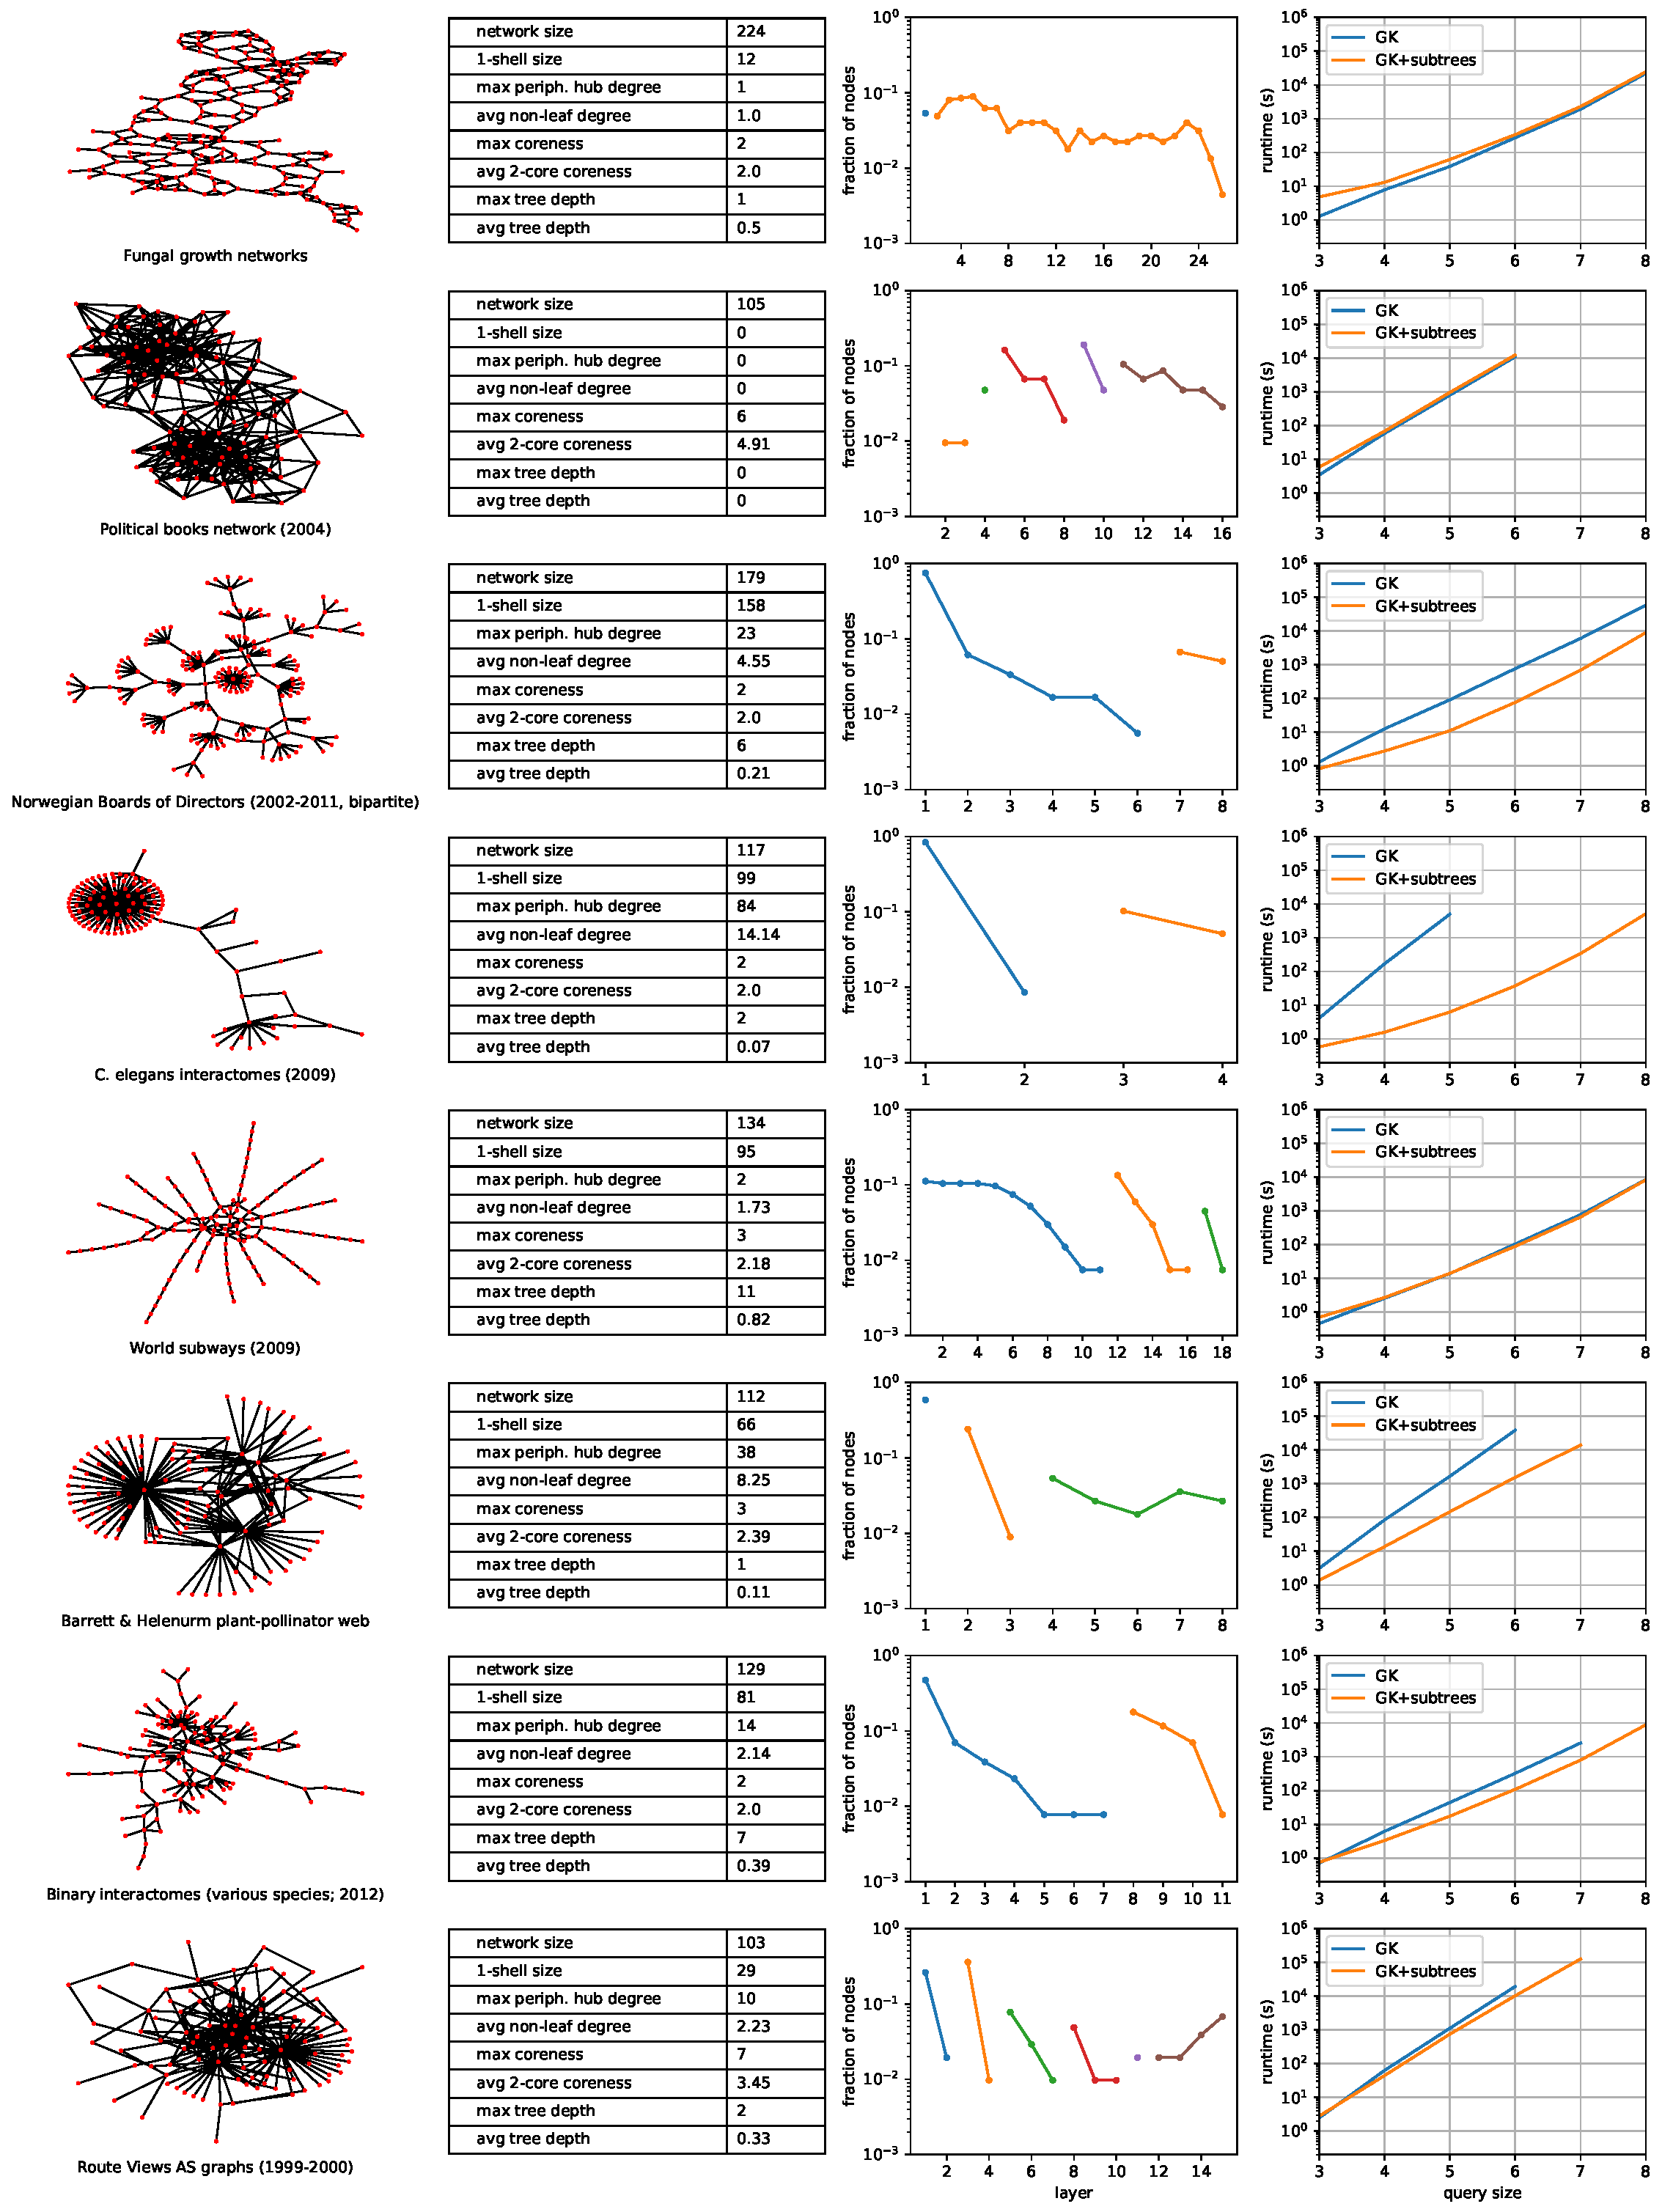
\includegraphics[width=15.6cm]{runtime_comparison_8sample}
	\caption{The first column shows each network from our sample. In the second column, \emph{max periph. hub degree} is the maximum degree of any vertex in the trees of the 1-shell, including their roots. The ``degree" of the root is taken as the number of adjacent vertices in the 1-shell. The third column shows the onion spectrum \cite{hebert2016multi} of each network, adn the last column shows a runtime comparison between our algorithm and the Grochow-Kellis symmetry-breaking algorithm.}
\end{figure}

\begin{figure}[h]
\label{fig:lsample_comparison}
	\centering
	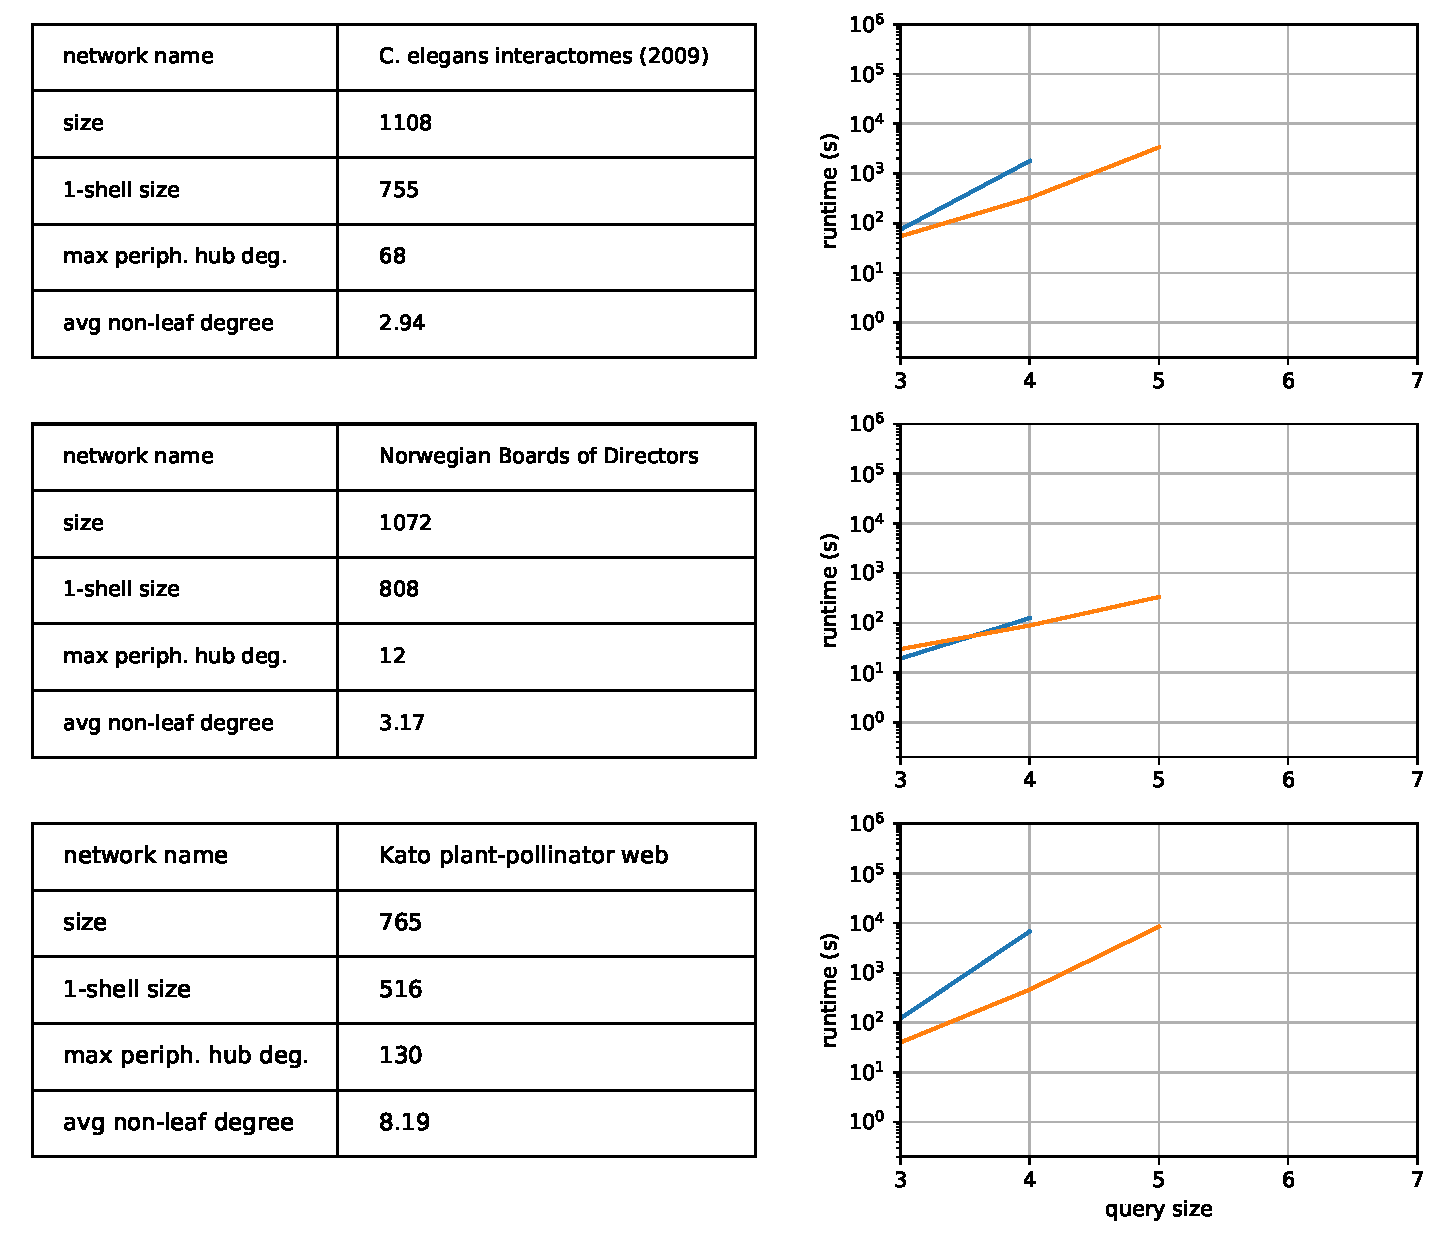
\includegraphics[width=10cm]{runtime_comparison_lsample}
	\caption{}
\end{figure}

\section{Conclusion}
\label{sec:conclusion}
We designed and implemented an algorithm for counting instances of a given graph in a network, leveraging tree and hub structure. Our study suggests that network and query topology can have a great impact on the runtime of motif search algorithms, and alleviates this problem in the case of trees. However, hubs are still major contributors to the complexity of motif search, whether they appear at the peripheries of a network or within the core. A more detailed analysis of the relationship between distribution of runtimes and topologies of query graphs could reveal the best angles of attack for more instance-aware algorithms, which we leave for future work.

\bibliographystyle{siamplain}
\bibliography{references}

% compile bibtex command: latex subtrees.tex && bibtex subtrees && latex subtrees.tex && latex subtrees.tex

\end{document}






